\documentclass{standalone}
\usepackage{pgfplots}
\begin{document}
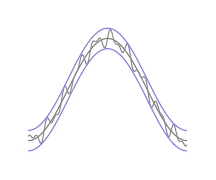
\begin{tikzpicture}
\pgfplotsset{width=4cm}
\begin{axis}[axis lines=none,scaled ticks=false]
\addplot[gray,domain=0:3.14159,samples=201]
{sin(deg(x))^2};
\addplot[gray!90!white,domain=0:3.14159,samples=201]
{sin(deg(x))^2+0.06*sin(20*deg(x))+0.04*cos(35*deg(x))};
\addplot[blue!50!white,domain=0:3.14159,samples=201]
{sin(deg(x))^2+0.1};
\addplot[blue!50!white,domain=0:3.14159,samples=201]
{sin(deg(x))^2-0.1};
\end{axis}
\end{tikzpicture}
\end{document}
